\chapter{INTRODUCTION}\label{chap1:introduction}


\begin{comment}


4. Multi-Sensory Reasoning-based ROSL Algorithm
4.1 Background
- how the problem is solved in biology (LLM forebrain, obstacle low(?)-brain)
    - Biology inspiration self-supervised learning models: MIT papers
    - Brief of which brain part does what, which one processes sensory inputs, comparable DL systems
    - How LLM is a brain-inspired candidate for navigation decision by reasoning over sensory inputs.
- proposed solution: generalized reasoning over detected objects with multimodal LLM
- how multimodal model works - not just object name, but with object context.
- the model is generalized, and has the ability to solve a specific problem
- related research (embodied AI and LLM based navigation)
- Hypothesis

5. Conclsion
- Summary of th entire paper
- Significance of the solutions
- Future research directions

\end{comment}

\section{Background}\label{Sec:1_background}
Sensory systems like olfaction, vision, and audition allow animals to interact with their surroundings. Of these, olfaction is the most ancient sensory system to evolve in organisms \cite{purves2001organization}. Olfaction enables organisms with odorant receptors to detect food, potential mates, threats, and predators \cite{sarafoleanu2009importance}. In some nocturnal mammals, such as mice, up to five percent of their genome is dedicated to olfaction \cite{ibarra2014olfactory}. 
% Olfaction in robotics
Similarly, a mobile robot with a chemical sensor can detect odors in the environment.

% \section{Problem Statement}\label{Sec:1_problemStatement}
Robotic odor source localization (ROSL) allows robots to mimic animals' olfaction-based behaviors. Specifically, it is the technology that allows robots to use olfaction sensory inputs to navigate toward an unknown target odor source in a given environment \cite{kowadlo2008robot}. %\textcolor{black}{Robotic} OSL  to accomplish a predetermined goal.
It has important applications, such as monitoring \mbox{wildfires \cite{wang2023vision}}, locating air pollution \cite{fu2019pollution}, detecting chemical gas leaks \cite{burgues2019smelling}, identifying unexploded mines and bombs \cite{russell2004robotic}, finding underground gas leaks \cite{chen2017underground}, and conducting marine surveys like locating hydrothermal vents \cite{wang20203}, among others.

Research on robotic odor source localization (OSL) has garnered considerable interest in recent decades \cite{jing2021recent}. Advancements in robotics and autonomous systems have enabled the deployment of mobile robots to locate odor or chemical sources.

%OSL algorithm: traditional olfaction-based approach
%This thesis describes the validation of a traditional ROSL algorithm in real-world environment, and then two proposed algorithms that incorporate vision sensing.

\section{Overall objectives}\label{Sec:overall_objectives}
% Objectives
\begin{figure}[h] %% figure

\ \\
\vspace*{-.18in}

\begin{center}
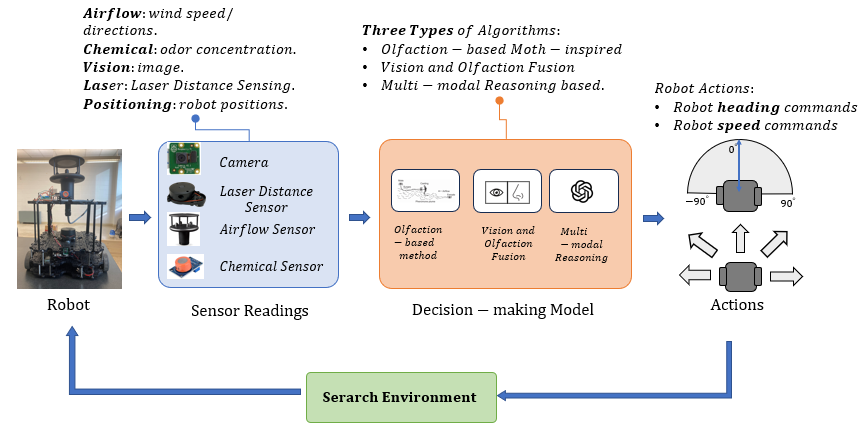
\includegraphics[width=0.99\columnwidth]{Main/Figure/objective.png}\hspace*{0.04in}
\end{center}
\vspace{-.1in}

\caption
{ROSL decision making model.}
%\end{singlespace}
\label{fig:overall_objective}
\end{figure}

Locating an unknown odor source necessitates an effective OSL algorithm to guide the robot based on sensor observations. \textcolor{black}{Figure~\ref{fig:overall_objective} shows the main decision-making loop of the ROSL system. The robot collects data from the environment using olfaction and vision sensors. In this work, the collected data is used by one of the three algorithms -}
\begin{itemize}
    \item traditional olfaction-based ROSL algorithm (detailed in chapter~\ref{chap:olfaction}).
    \item proposed vision and olfaction fusion ROSL algorithm (detailed in chapter~\ref{chap:fusion}).
    \item proposed multi-modal reasoning-based ROSL algorithm (detailed in chapter~\ref{chap:LLM}).
\end{itemize}
The navigation algorithm calculates the robot heading for localizing the odor source. The robot heading is executed by the robot, which changes its environment state. The robot again collects data and the loop continues till it localizes the odor source.

The thesis is divided into three main chapters. The main goal of chapter~\ref{chap:olfaction} is to discuss the development of a robot platform that can be used to validate a traditional ROSL algorithm. The chapter includes -
\begin{itemize}
    \item review of recent progress of ROSL research;
    \item discussion of the development of a multi-modal robot platform for real-world experimentation, and;
    \item discussion of real-world experimentation for the validation of a traditional olfaction-only ROSL navigation algorithm.
\end{itemize}

Chapter~\ref{chap:fusion} introduces a novel ROSL navigation algorithm. It proposes the incorporation of vision sensing for ROSL navigation. The chapter includes -
\begin{itemize}
    \item discussion of the limitations of traditional olfaction-based ROSL approach;
    \item discussion of the incorporation of deep-learning-based vision sensing in ROSL with the proposed vision and olfaction fusion navigation algorithm. 
    \item real-world ROSL performance comparison of traditional olfaction-only and the proposed fusion method.
\end{itemize}

Chapter~\ref{chap:LLM} proposes the application of multi-modal LLM for zero-shot ROSL navigation. The chapter includes -
\begin{itemize}
    \item discussion of the limitations of supervised vision processing.
    \item discussion of using multi-modal Large Language Model (LLM) as the zero-shot decision maker in ROSL navigation algorithm.
    \item real-world performance comparison of the validated vision and olfaction fusion navigation algorithm with a multi-modal reasoning-based navigation algorithm.
\end{itemize}

Finally, chapter~\ref{chap:conclusion} summarizes the significance of the work.

